\begin{enumerate}[label=\thesection.\arabic*.,ref=\thesection.\theenumi]
\numberwithin{equation}{enumi}

\item
What is the purpose of a phase lead compensator?

\solution 
\begin{itemize}
    \item Phase lead compensators are used to produce an output having a phase lead when an input is applied
    \item The major application is to help improve the Phase Margin (P.M) of the system.
\end{itemize}

\item
Through an example show how the compensator in Problem 7.1 can be used in a control system

Consider a control system with the Transfer Function

\begin{align}
G(s) = \frac{1}{s(3s+1)}
\end{align}
\begin{align}
G\brak{\j\omega}&=\frac{1}{\brak{j\omega}\brak{3j\omega+1}} 
\end{align}

\begin{align}
\implies 
\abs{G\brak{\j\omega}}&=\frac{1}{{\omega}{\brak{\sqrt{9\omega^2+1}}}}
\end{align}

\begin{align}
\angle G\brak{\j\omega}&=- \tan^{-1}(3\omega) - 90\degree
\end{align}

At Gain Crossover,
\begin{align}
\abs{G\brak{\j\omega}}&=1
\end{align}

\begin{align}
\implies \frac{1}{{\omega}{\brak{\sqrt{9\omega^2+1}}}} =1
\end{align}

\begin{align}
\implies \omega_{gc} = 0.531
\end{align}

\begin{align}
\angle G\brak{\j\omega} = -147.88\degree
\implies PM=32.12\degree
\end{align}
Phase Margin is only 32.12\degree which is below the acceptable range of Phase Margin i.e 45\degree.

Now we will apply Lead Compensator
\begin{align}
D(s) = \frac{3(s+\frac{1}{3T})}{(s+\frac{1}{T})}
\end{align}
Choose T = 1 for this compensator

We have,
\begin{align}
D(s) = \frac{3(s+\frac{1}{3})}{(s+1)}
\end{align}

By cascading the Compensator and the Open Loop Transfer Function, we get
\begin{align}
D(s)G(s) = \frac{1}{s(3s+1)} \frac{3(s+\frac{1}{3})}{(s+1)}
\end{align}

\begin{align}
Let G_{1}(s) = D(s)G(s)
\end{align}

\begin{align}
\implies G_{1}(s) = \frac{1}{s(s+1)}
\end{align}

Calculating Phase Margin for cascaded Transfer Function
\begin{align}
G_{1}(s) = \frac{1}{s(s+1)}
\end{align}
\begin{align}
G_{1}\brak{\j\omega}&=\frac{1}{\brak{j\omega}\brak{j\omega+1}} 
\end{align}

\begin{align}
\implies 
\abs{G_{1}\brak{\j\omega}}&=\frac{1}{{\omega}{\brak{\sqrt{\omega^2+1}}}}
\end{align}

\begin{align}
\angle G_{1}\brak{\j\omega}&=- \tan^{-1}(\omega) - 90\degree
\end{align}

At Gain Crossover,
\begin{align}
\abs{G_{1}\brak{\j\omega}}&=1
\end{align}

\begin{align}
\implies \frac{1}{{\omega}{\brak{\sqrt{\omega^2+1}}}} =1
\end{align}

\begin{align}
\implies \omega_{gc} = 0.786
\end{align}

\begin{align}
\angle G\brak{\j\omega} = -128.167\degree
\implies PM=51.83\degree
\end{align}

As we can see, the Phase Margin has gone above 45\degree which is the acceptable range of Phase Margin.

Therefore, through this example we have shown that a Lead Compensator is helpful in improving the Phase Margin of the System.

\item Verify the above improvement in Phase Margin with the help of a Python Code
\solution
\begin{lstlisting}
codes/EE18BTECH11021_2.py
\end{lstlisting}

\begin{figure}
\centering
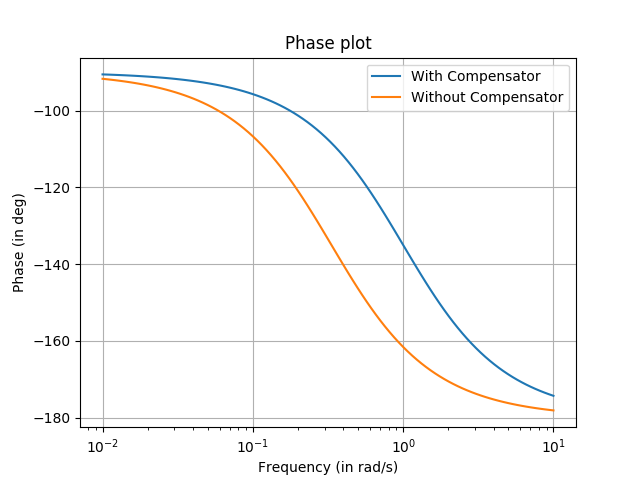
\includegraphics[width=\columnwidth]{figs/EE18BTECH11021_fig_2.png}
\end{figure}
